
\subsection{Timeline}

Time stamps are used to allocate events to a specified time.
With the help of these time stamps a timeline can be created. 
In this timeline you can see which action was done to an object at a specific time and which action followed after a specific action. 
The timeline also  represents, what kind of action (created, modified, accessed) had taken place. 
Time stamps can be found in different metadata like in file system, application, log data and many other data. 
Metadata are information about entities and are usually stored with the digital object. 
In different digital objects you can find different metadata. 
For example in a photo you find other metadata as in a word document. 
In a photo you can find information like the ISO value and exposure time, which you can not find in a word document. 
The important metadata for the timeline are the different times. 
These time stamps are called MACtimes. 
The MAC abbreviation stands for the following. 
M stands for the modified time (mtime), a  stands for the accessed time (atime) and c stands for the changed time (ctime). 
It can happen that all of these show the same value. 
The access time is the time at which the file was read the last time. 
The modify time shows the last time content was written.
The change time reflects the time at which the file metadata was changed, for example a file got another permission or owner. 
NTFS, the file system of current Windows versions, offers a fourth time, which is called born time (btime). 
This represents when the object was created.
The born time is not available in Ext2 and Ext3. 
In Table~\ref{fig:Mactimes} you can see the meaning of MACtimes in different file systems. 

\begin{table}[h]

\begin{tabular}{c|c|c|c|c}
	File System & modified & accessed & changed & birth \\
	\hline \hline
	Ext2/3 & modified & accessed & changed & N/A \\
	\hline
	FAT & written & accessed & N/A & created \\
	\hline
	NTFS & file modified & accessed & MFT modified & created \\
	\hline
	UFS & modified & accessed & changed & N/A \\

\end{tabular}

\caption{Mactimes}
\label{fig:Mactimes}
\end{table}

Using this information we retraced the suspects steps and created a timeline which can be seen in figure~\ref{fig:timeline}.
At first the criminal loaded files from the internet with illegal content. 
Then a Truecrypt-container (setup.exe) was created and changed. 
Changed means in this context that he probably added data to the container.
After that the criminal accessed the data and read it. 
Later, two other Truecrypt container were created. 
We got these various time stamps with the help of the tool “Redline”. 
A timeline is used to reconstructed the order of actions the suspect did, which includes objects created, accessed or modified.

Different problems can occur during the analysis of the timeline.
A problem in the NTFS file system is that it can take up to one hour to update the corresponding time stamp after it was accessed.\foodnote{FileTimes} 
Furthermore, a criminal can change the MACtime values on purpose to obscure examiners. 
One program which can change the time stamps is named BulkFileChanger\foodnote{http://www.nirsoft.net/utils/bulk_file_changer.html} by NirSoft.
BulkFileChanger can overwrite the create, modify and access time. 
One more problem which exists is that sometimes it is difficult to know if an object was accessed by an application or a person. 
All of these issues need to be considered in order to get an accurate result. 

There are important hints for a digital investigator. 
These hints can tell what happened with a file. 
The digital investigator can recognize through the combination of Mactimes which actions happened to a file, e.g. if the modified time is before the created time, then the file was copied from one system or moved from one partition to another partition. 
More of these methods are described in \foodnote{alazab2009effective}.

\begin{figure}[tbph]
	\centering
		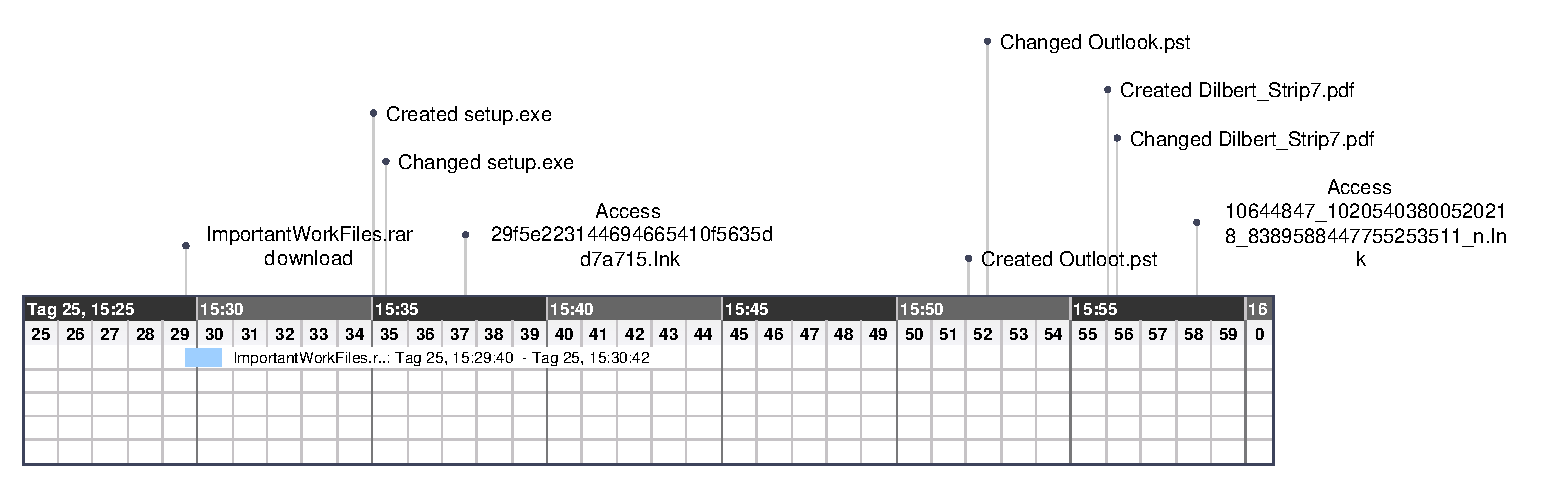
\includegraphics[width=\textwidth]{graphics/Timeline.pdf} 	
	\caption{Timeline}
	\label{fig:timeline}
\end{figure}
